% UC3M + ISCIII report template. English version of main.tex: same
% package, same layout; the only change is the babel line below. Demo of
% the title block with subject/degree/group/professor, sections and
% subsections, a list, a table, a figure, a formula, links and a bibtex
% bibliography (its "References" heading comes from babel-english).
%
% Build:  make      (latexmk -lualatex, two passes for \pageref{LastPage};
%                    produces build/main-en.pdf along with the Spanish demo)
%
% No inputenc/fontenc needed: under LuaLaTeX+fontspec the engine handles
% the encoding, and loading them here would only produce warnings.
\documentclass[11pt,twoside]{article}

% babel goes BEFORE uc3misciidoc: the package loads hyperref internally,
% and hyperref needs babel already active to pick the right \autoref names.
% The package has no language option: it detects whether babel is set to
% Spanish and only then applies its babel-spanish tweaks; with english (or
% no babel at all) everything is left as LaTeX/babel provide it.
\usepackage[english]{babel}
% hyperref's English defaults for \autoref are "Table 1"/"Figure 1" but a
% lowercase "section 2". To capitalise it, uncomment the line below (it
% must go through \extrasenglish: babel re-applies hyperref's names at
% \begin{document}, so a plain \renewcommand in the preamble is lost).
% \addto\extrasenglish{\renewcommand{\sectionautorefname}{Section}}
\usepackage{uc3misciidoc}

\title{Performance analysis of a distributed queueing system}
\subject{Distributed Systems}
\degree{Bachelor in Computer Science and Engineering}
\group{Group 81}
\professor{Pedro Pedro Pedro}
\author{Raúl Aguilar Arroyo \and Raúl Aguilar Arroyo}
\date{Academic year 2026/2027 -- First semester}
\shorttitle{Distributed queue performance}

\begin{document}
\maketitle

\section{Introduction}

This document reports the performance analysis of a distributed queueing
system under different load levels, carried out as the course report for
the subject shown in the title block.

\subsection{Goals}

The aim is to characterise the latency and throughput of the system as a
function of the number of active producers and consumers, and to identify
the point beyond which the error rate stops being negligible.

\subsection{Document structure}

The experimental design is described in \autoref{sec:methodology};
the results obtained are presented in \autoref{sec:results};
\autoref{sec:conclusions} summarises the conclusions.

\section{Methodology}
\label{sec:methodology}

\subsection{Experimental design}

A three-node cluster was deployed to run the queueing system, generating
synthetic load with different request-arrival profiles.

\subsubsection{Simulation parameters}

The parameters considered in each configuration were:

\begin{itemize}
  \item Number of concurrent producers.
  \item Number of concurrent consumers.
  \item Maximum queue size.
  \item Retry policy under saturation.
\end{itemize}

\section{Results}
\label{sec:results}

\autoref{tab:results} summarises the mean response times and the
throughput observed in each configuration evaluated.

\begin{table}[h]
  \centering
  \caption{Mean response times per configuration.}
  \label{tab:results}
  \begin{tabular}{@{}lrrr@{}}
    \toprule
    Configuration & Latency (ms) & Throughput (req/s) & Error (\%) \\
    \midrule
    Low load     & 12  & 480  & 0.0 \\
    Medium load  & 34  & 1120 & 0.2 \\
    High load    & 97  & 1780 & 1.8 \\
    Saturation   & 310 & 1825 & 9.4 \\
    \bottomrule
  \end{tabular}
\end{table}

\autoref{fig:latency} shows how the response time evolves as the load on
the system increases.

\begin{figure}[h]
  \centering
  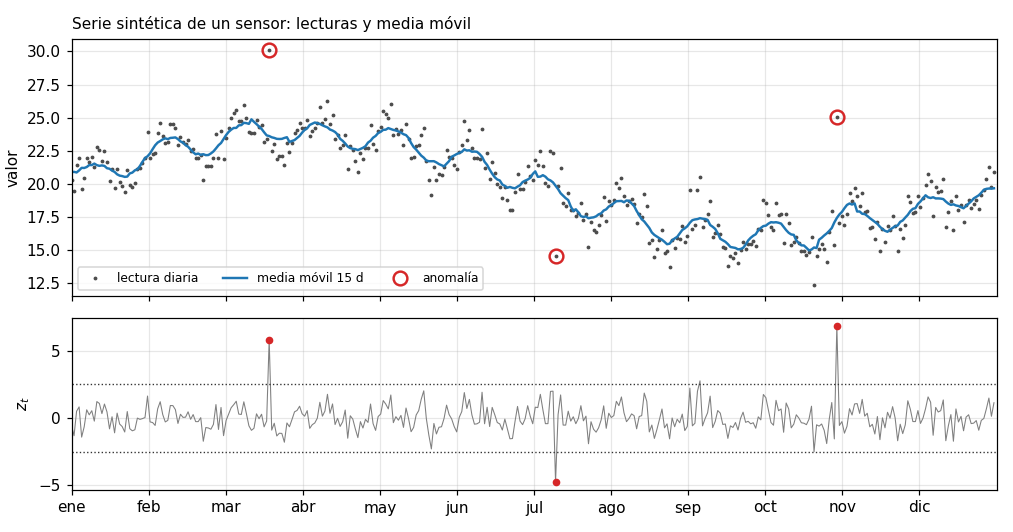
\includegraphics[width=0.7\linewidth]{figs/demo-figura}
  \caption{Response time under increasing load.}
  \label{fig:latency}
\end{figure}

The mean waiting time in an M/M/1 system is given by
\[
  W = \frac{\rho}{\mu - \lambda},
\]
where $\lambda$ is the arrival rate, $\mu$ the service rate and
$\rho = \lambda / \mu$ the system utilisation~\cite{kleinrock1975}.

The data were collected with the Locust tool\footnote{See
\url{https://locust.io}.} on the cluster described in
\autoref{sec:methodology}.

\section{Discussion}
\label{sec:discussion}

The results are consistent with what is expected for an M/M/1 queueing
system: latency grows sharply as the system utilisation approaches one,
whereas throughput levels off well before that limit. This behaviour is
also the one expected in a distributed system where nodes communicate
through queues~\cite{tanenbaum2007}.

\subsection{Limitations of the study}

The experiment was run with a single request-arrival profile (homogeneous
Poisson). A more realistic profile with traffic bursts would probably
bring forward the saturation point observed in \autoref{sec:results}.

The effect of partial cluster failures (loss of one of the three nodes)
was not evaluated either; it could degrade performance far more abruptly
than a plain increase in load.

\subsection{Future work}

As a natural continuation of this work, we propose repeating the
experiment with a load generator that includes bursts, and adding a
node-failure scenario to characterise service degradation under
conditions closer to a real production environment.

\section{Conclusions}
\label{sec:conclusions}

The system keeps a negligible error rate up to the high-load
configuration; beyond that point, response time grows non-linearly and
the error rate is no longer acceptable, which places the practical
operating limit just below the saturation regime.

\bibliographystyle{plain}
\bibliography{referencias}

\end{document}
